\documentclass{beamer}

\usefonttheme{professionalfonts} % using non standard fonts for beamer
\usefonttheme{serif} % default family is serif

\usepackage{hyperref}

%\usepackage{minted}

\usepackage{animate}

\usepackage{graphicx}

\def\Put(#1,#2)#3{\leavevmode\makebox(0,0){\put(#1,#2){#3}}}

\usepackage{color}

\usepackage{tikz}

\usepackage{amssymb}
\usepackage{amsthm}

\usepackage{enumerate}


\newcommand\blfootnote[1]{%

  \begingroup

  \renewcommand\thefootnote{}\footnote{#1}%

  \addtocounter{footnote}{-1}%

  \endgroup

}

\makeatletter

%%%%%%%%%%%%%%%%%%%%%%%%%%%%%% Textclass specific LaTeX commands.

 % this default might be overridden by plain title style

 \newcommand\makebeamertitle{\frame{\maketitle}}%

 % (ERT) argument for the TOC

 \AtBeginDocument{%

   \let\origtableofcontents=\tableofcontents

   \def\tableofcontents{\@ifnextchar[{\origtableofcontents}{\gobbletableofcontents}}

   \def\gobbletableofcontents#1{\origtableofcontents}

 }

%%%%%%%%%%%%%%%%%%%%%%%%%%%%%% User specified LaTeX commands.

\usetheme{Malmoe}

% or ...

\useoutertheme{infolines}

\addtobeamertemplate{headline}{}{\vskip2pt}

\setbeamertemplate{theorems}[numbered]

\theoremstyle{definition}
\newtheorem{defn}{Definition}[section]

\setbeamercovered{transparent}

% or whatever (possibly just delete it)

\makeatother

\begin{document}
\title[]{Update}
\author[Update]{Andres}
\institute[]{University of California, Riverside}
\makebeamertitle
\newif\iflattersubsect

\AtBeginSection[] {
    \begin{frame}<beamer>
    \frametitle{Outline} 
    \tableofcontents[currentsection]  
    \end{frame}
    \lattersubsectfalse
}

\AtBeginSubsection[] {
    \begin{frame}<beamer>
    \frametitle{Outline} 
    \tableofcontents[currentsubsection]  
    \end{frame}
}

\section{Algorithms}

\begin{frame}{Algorithms}
    \begin{itemize}
        \item Split the problem in two stages: 
            \begin{enumerate}
                \item Find maximal disks at each timestamp (MaximalFinder) and
                \item Join maximal disks between adjancent timestamps (FlockFinder)
            \end{enumerate}
        \item Pseudocode for both algorithms available online: {\color{blue}\href{https://github.com/aocalderon/Research/raw/master/Docs/MeetingPTs/MF-Pseudocode.pdf}{MaximalFinder\footnote{\url{https://tinyurl.com/y74lld5k}}}} and {\color{blue}\href{https://github.com/aocalderon/Research/raw/master/Docs/MeetingPTs/FF-Pseudocode.pdf}{FlockFinder\footnote{\url{https://tinyurl.com/yac26guf}}}}.
    \end{itemize}
\end{frame}

\begin{frame}{Maximal finder overall steps}
    \begin{enumerate}
        \item Indexing points...
        \item Getting pairs...
        \item Computing centers...
        \item Indexing centers...
        \item Getting disks...
        \item Filtering disks $<\mu$...
        \item Prunning duplicate candidates...
        \item Indexing candidates...
        \item Getting expansions...
        \item Finding maximal disks.
    \end{enumerate}
\end{frame}

\begin{frame}{Flock finder}
    \begin{enumerate}
        \item Set of disks for $t_i$...
        \item Set of disks for $t_{i+\delta}$...
        \item Joining timestams...
        \item Checking internal timestamps.
    \end{enumerate}
\end{frame}

\section{Performance evaluation}

\begin{frame}{Performance}
    \centering
    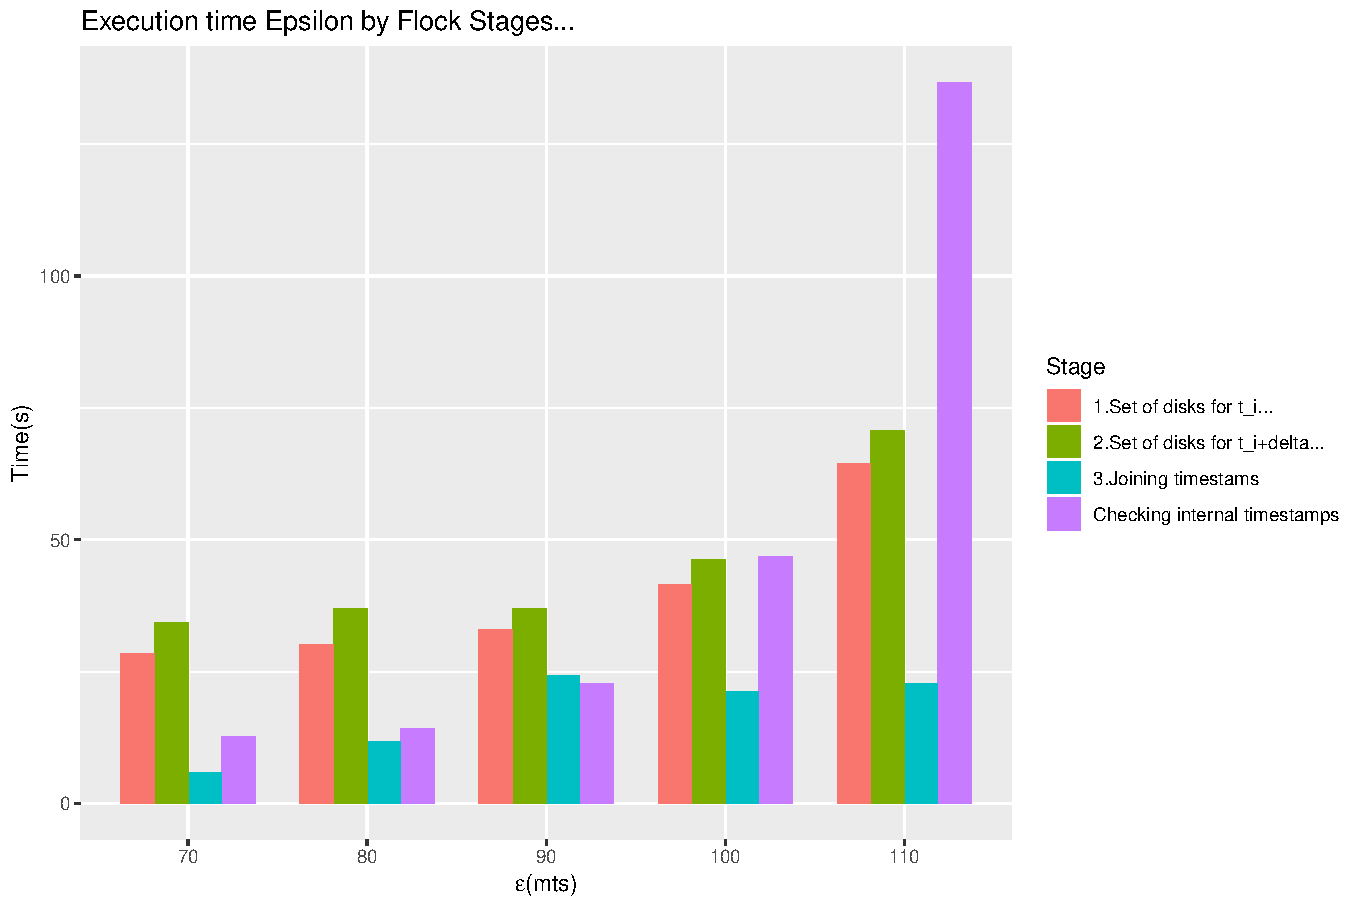
\includegraphics[width=0.9\textwidth]{MergeLastFlocksByStage}
\end{frame}

\begin{frame}{Performance}
    \centering
    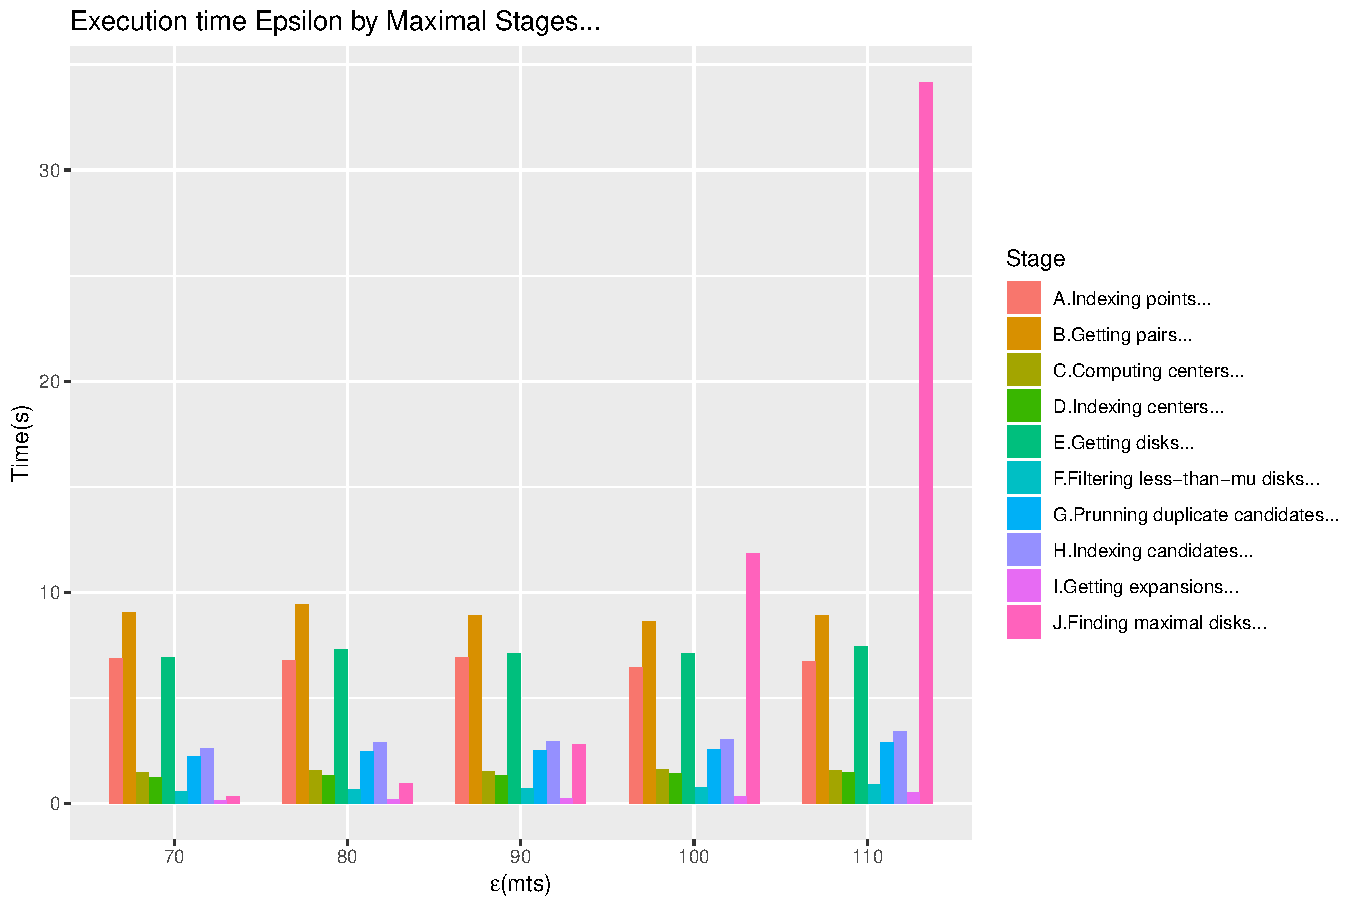
\includegraphics[width=0.9\textwidth]{MergeLastMaximalsByStage}
\end{frame}

\begin{frame}{Performance}
    \centering
    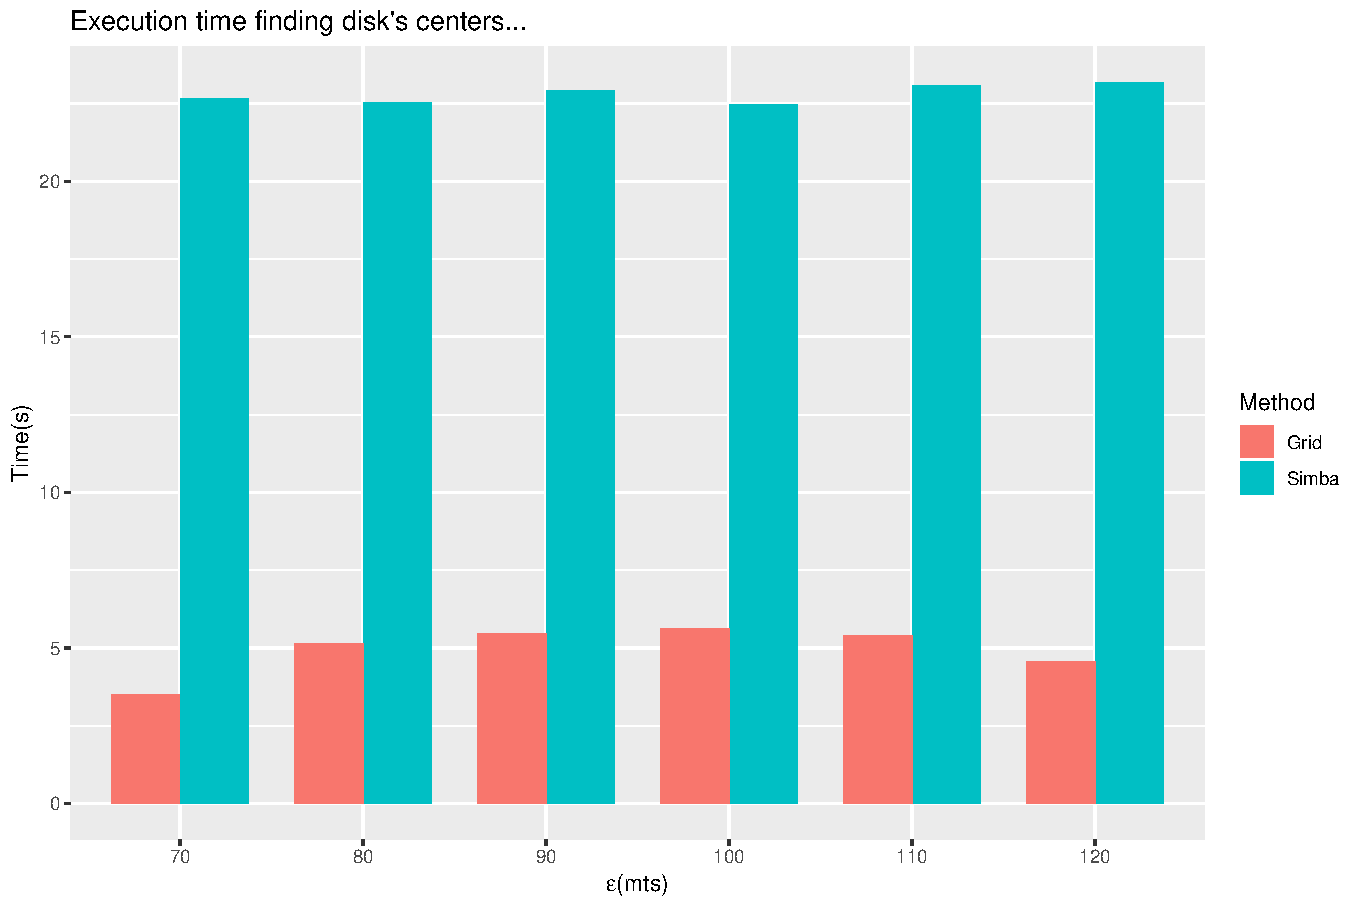
\includegraphics[width=0.9\textwidth]{Indexing}
\end{frame}

\begin{frame}{Bottlenecks}
    \begin{enumerate}
        \item In flock finder:
            \begin{itemize}
                \item Checking internal timestamps: When merge last approach prunes enough points it works as expected but large amount of intermediate points have huge impact. 
            \end{itemize}
        \item In maximal finder:
            \begin{itemize}
                \item Finding maximal disks: Even the new implementation is more stable, the most costly operation is removing duplicates and redundant disks.
            \end{itemize}
        \item Overall:
            \begin{itemize}
             \item Online approach requires indexing at each timestamp.
             \item Simba indexing is slow.
            \end{itemize}
    \end{enumerate}
\end{frame}

\section{Possible solutions}

\begin{frame}{Possible solutions}
    \begin{enumerate}
        \item Explore alternatives in Simba\footnote{Already done.}
        \begin{itemize}
            \item There are QuadTree and KDTree partitioners but they are not fully-integrated as indeces. (QuadTree only support 2D.)
            \item For partitioning, RTree is already faster than QuadTree and KDTree in 2D and 3D datasets.   
        \end{itemize}

        \item Grid indexing
        \begin{itemize}
            \item Include the Grid partitioner in Simba and work on its index integration.
            \item Implement distance join by my own.
        \end{itemize}

    \end{enumerate}
\end{frame}

\section*{Extra slides}

\begin{frame}{Grid partitioning}
    \centering
    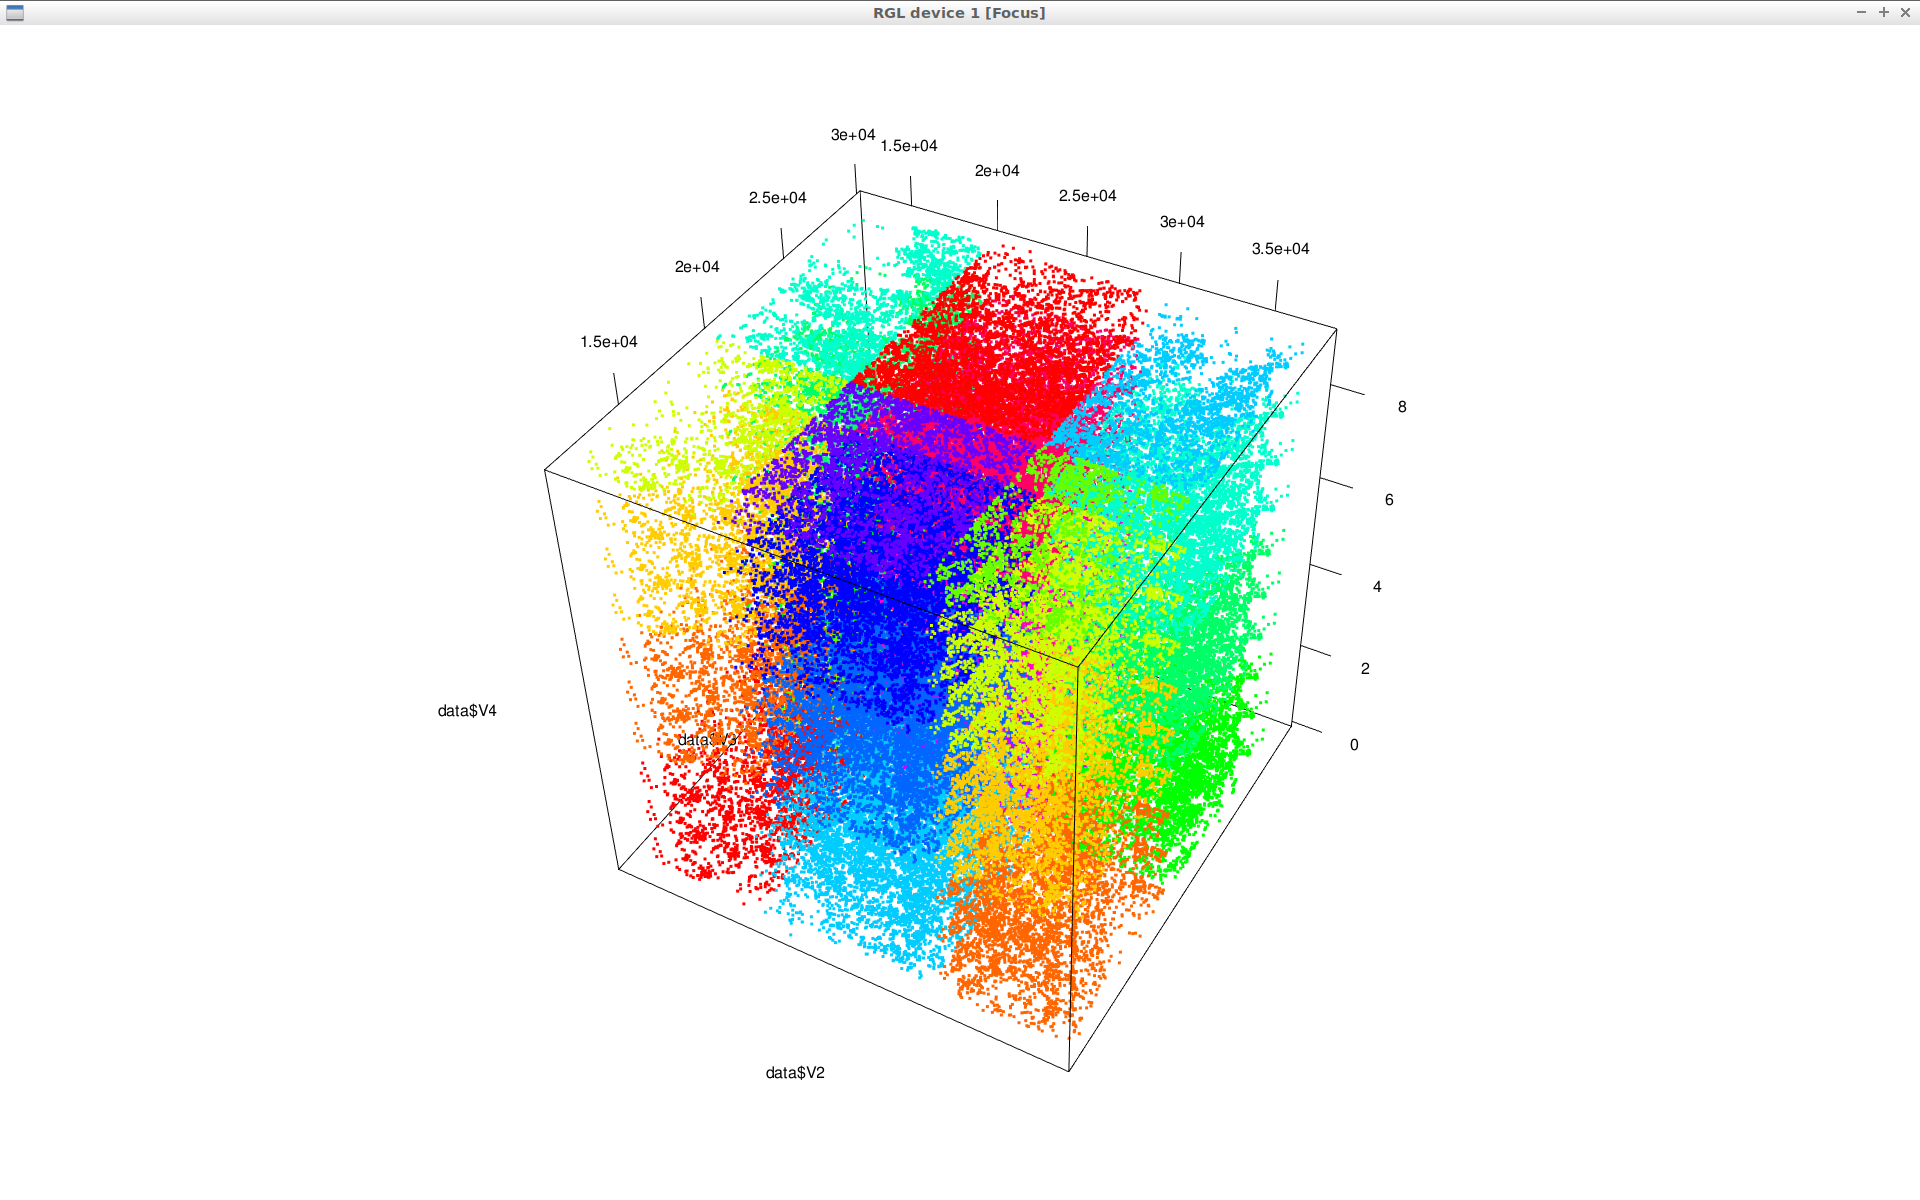
\includegraphics[trim={4cm 4cm 4cm 4cm},clip,width=\textwidth]{grid3d}
\end{frame}

\begin{frame}{Grid partitioning}
    \centering
    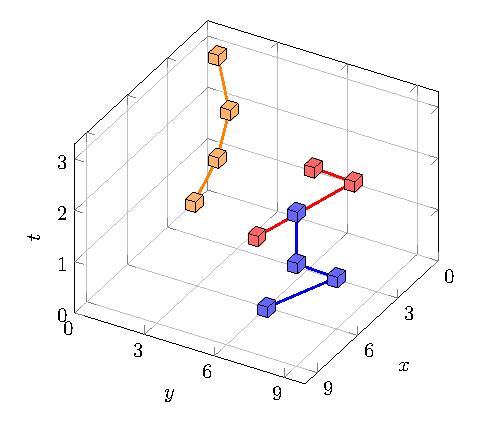
\includegraphics[width=0.9\textheight]{cube}
\end{frame}

\end{document}
